\section{Projektentwicklung}
\label{sec:development}

\subsection{Usecases}

\subsubsection{Login}

Ein Fahrer hat im System einen Benutzer. Durch Benutzername und Passwort kann sich der Fahrer auf dem Android-System einloggen. Als Authentifizierungssystem zum Server werden dabei CouchDB-User verwendet. Details zum Authentifizierungssystem sind unter Abschnitt \ref{sec:security}.

Nach dem Einloggen kann der Fahrer sein Fahrzeug wählen. Das Auswählen des Fahrzeuges ist notwendig, damit das Android-System weiß welche Sensoren auszulesen sind. In Kapitel \ref{sensors} ist beschrieben wie jedes Fahrzeug mit Sensoren ausgestattet wird. 

In Abbildung \ref{fig:login} ist ersichtlich wie der Loginvorgang durchgeführt wird. Nach dem Loginvorgang versucht das System eine Anfrage für neue Daten an den Server zu senden.  Bei einer aktiven Serververbindung werden die Benutzerdaten und das gewählte Fahrzeug an den Server gesendet. Nach einer Authentifizierung des Benutzers wird ermittelt ob für das gewählte Fahrzeug neue Daten bezüglich der Sensoren vorhanden sind. Sind neue Daten vorhanden werden diese per Datenbankreplikation an das mobile Gerät gesendet.

Bei der Replikation werden Container-Dokumente übertragen. In diesen Dokumenten sind die Informationen gespeichert, welche Sensoren auf dem jeweiligen Fahrzeug vorhanden sind und wie diese anzusprechen sind.

\begin{figure}
	\centering
		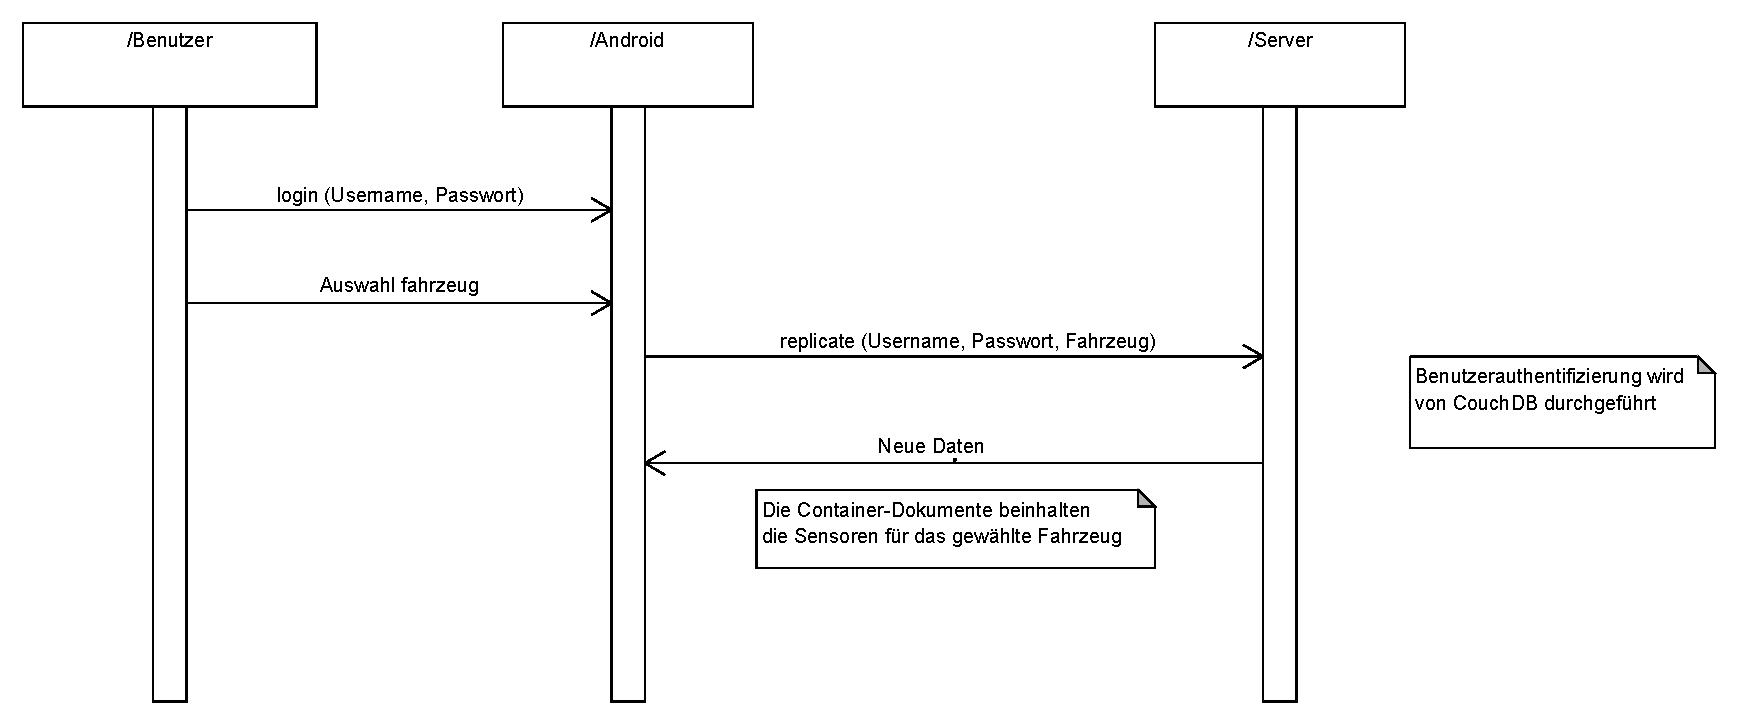
\includegraphics[width=\textwidth]{files/pdf/Login.pdf}
	\caption{Loginvorgang}
	\label{fig:login}
\end{figure}


\begin{itemize}
  \item Wareneingang
  	\subitem registriert Pakete im System
  	\subitem klebt QR-Code auf Pakete

	\item Logister plant und erstellt Lieferungen (neue Auftragsnummer wird
	generiert) \subitem wählt Pakete aus (können mit Sensoren bestückt sein)
		\subitem wählt Fahrer aus 
		\subitem wählt Transportmittel (können mit Sensoren bestückt sein) für
		Lieferungen aus
		\subitem trägt Zielort und Auftraggeber ein
  	
  \item Transporteur
  	\subitem holt oder hat Device mit Roadrunner App
  	\subitem loggt sich im Roadrunner System ein
  		\subsubitem mit Benutzerdaten wird sein/e aktuelle/r Auftrag/Lieferung aufs
  		Device synchronisiert ODER 
  		\subsubitem scannt Pakete und lädt sie in das vom Logistiker ausgwählte
  		Transportmittel
\end{itemize}

\paragraph{Daten-Synchronisierung}
	\textbf{Vorbedingungen: }
	\begin{itemize}
	  \item Transporteur hat sich in der System-App eingeloggt
	\end{itemize}
	
	Die Daten-Synchronisierung oder Replizierung wird durch das Einloggen im
	System angestoßen. Das mobile Gerät erhält folgende Information:
	\begin{itemize}
	  \item Adressen der Sensoren, die das Gerät überwachen sollte
	  \item alle Produkte, Pakete der aktuellen Lieferung, sowie Zielort, etc.
	  \item Überwachungs-Thresholds der Pakete
	\end{itemize}
\par

\subsection{Iteration 1}

\subsubsection{Ziele}

\begin{itemize}
  \item Produkte können erzeugt werden.
  \item Produkte können eingelagert werden.
  \item Produkte können ausgelagert werden.
\end{itemize}

\subsubsection{UML}

\begin{figure}
	\centering
		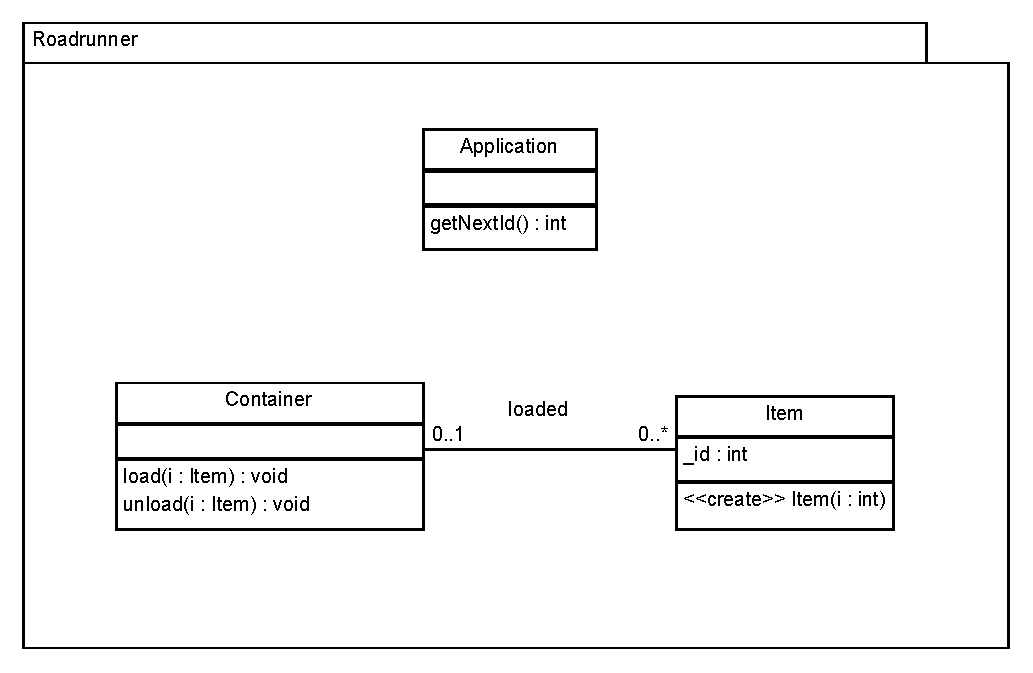
\includegraphics[width=\textwidth]{files/pdf/Iteration1.pdf}
	\caption{Iteration 1}
	\label{fig:Iteration1}
\end{figure}
